\documentclass[a4paper,10pt,twocolumn,twoside]{article}
\usepackage{fullpage}
\usepackage{graphicx}
\usepackage{pgfplots}
\usepackage{pgfplotstable}
\usepackage{filecontents}
\usepackage{booktabs}
\usepackage{tabularx}
\usepackage{tikz}
\usepackage{listings}
\usepackage{authblk}
\usepackage{caption}
\usepackage{mathtools}

\usetikzlibrary{patterns,shapes,positioning,calc}

\lstset{language=C, basicstyle=\ttfamily\small, columns=flexible}

\pgfplotsset{compat=1.8}

\author{Lars Kirkholt Melhus}
\author{Rune Erlend Jensen}
\affil{Norwegian University of Science and Technology}
\title{Sources of Measurement Bias in Modern CPUs}
\date{} % This is a timeless piece

\begin{document}

\twocolumn[
  \begin{@twocolumnfalse}
    \maketitle
    \begin{abstract}
    Seemingly innocuous properties of the execution context, such as the contents of system environment variables, or variations in link ordering, can impact the performance of computer programs. 
    Variations in external properties like these can bias programs towards certain configurations. 
    These effects have been shown to be a significant issue in performance analysis, but unpredictable and difficult to deal with.

    Abstract This paper focuses on the underlying reasons for bias effects that can be experienced for example by changing environment variables, or using different link orders. 
    Through experimentation and careful measurements using performance counters, we identify several potential sources of bias on the 4th generation Intel Core i7 architecture Haswell. 
    Limitations imposed by the Loop Stream Detector is revealed, along with effects from 4K address aliasing. We show that bias is in fact not completely unpredictable, and discuss measures for avoiding it.
    \end{abstract}
    \bigskip
        
  \end{@twocolumnfalse}
]


\section{Introduction}
Optimizing for performance is an important topic in computer science, and high performance computing (HPC) in particular. 
A great amount of research and effort is put into designing better algorithms and compiler optimizations, in order to produce an “optimal” executable. 
However, performance of computer programs is not just a function of the collection of machine instructions executed. 
Various external properties, such as the operating system and user environment, can have have an impact on how fast programs execute. 
Characteristics of the operating system can decide things like the placement of code and data in memory, which in turn interacts with various hardware mechanisms. 
Corner cases in hardware introduces potential performance cliffs; If for example a memory access happens to cross a page boundary, the cost of an additional TLB miss can be significant. 
The set of conditions under which a program executes is called the execution context, which includes virtual memory layout in particular. 
Variations within contexts can lead to programs being biased towards certain configurations. 
Measuring performance of the same program on two machines with identical hardware can sometimes yield very different results, an effect known as measurement bias.

Previous work has studied parameters such as the size of Unix environment variables and program link order. 
Both are found to potentially have a significant effect on performance, even in standardized benchmarks. 
Unfortunately, the effects also appear to be unpredictable, and therefore difficult to deal with. 
This poses a problem for researchers and performance analysts, who will need to account for effects of measurement bias with more rigorous methodologies and statistical methods.

Both the size of environment variables and link ordering ultimately has an effect on memory layout of running processes. 
We will not look at things like cache efficiency, which often can be the reason for bad performance under certain memory contexts. 
Instead, we look at effects from less known optimizations in the out-of-order execution engine and instructions fetch pipeline. 
Because bias effects are intrinsically connected to various hardware features, this paper is focued on the Intel® Core™ i7 “Haswell” architecture specifically. 
However, the bias sources we present has also been shown to behave similarly on previous Intel architectures as well.
With a better understanding of intricate properties of the CPU, we show how one is able to not only predict, but also explicitly optimize for beneficial memory layouts. 

In the paper appropriately named “Producing Wrong Data Without Doing Anything Obviously Wrong” by T. Mytkowicz et al.~\cite{Mytkowicz:2009:WrongData}, the authors show how simple changes to the execution environment can have an impact on performance. 
One of their examples is a program where performance varies significantly with changes to the environment variables. 
Unix environment variables contain various information about the system, such as the name of the currently logged in user, home- and current directory path.
This means that the length of your name -- by extension you user login -- could in principle be the tipping point between good and bad performance.

Previous work focuses mostly on how to mitigate effects of bias, and avoid drawing the wrong conclusions based on misleading measurements~\cite{Mytkowicz:2008:Easy, Mytkowicz:2009:WrongData}.
The goal of this paper is to show not only that bias exists, but also \emph{why} it occurs. 

With more accurate models of how bias occur, we will not only be able to actively avoid in performance, but in some cases also gain a real speedup on average.

Modern microprocessors are extremely complex in design and functionality. 
Some features of recent Intel processors includes several layers of cache to camouflage slow memory, multiple prefetchers, speculative out-of-order execution and branch prediction, just to name a few.
Hardware features and optimizations interact with memory layout of program code and data in various ways.
We will unveil characteristics about two different architectural features in recent Intel CPUs, and show how they can bias performance towards certain memory contexts. 

First we will look at an aliasing effect between memory addresses of loads and stores, causing false dependencies in the out-of-order execution pipeline. 
This effect can be triggered for example by changing stack position, and can explain bias from altering environment variables. 
Secondly, we will look at the Loop Stream Detector, which in previous work on measurement bias has been suggested as a possible explanation.
We therefore choose to study this particular optimization in detail, and show how measurement bias can occur from changing link order.


\section{Methodology}
When studying bias effects, carefully controlling all relevant properties of the environment is crucial. 
Previous work on measurement bias and observer effect describes a set of best practices for how the measurement infrastructure should be configured \cite{Mytkowicz:2009:WrongData, Mytkowicz:2008:OE&MB}. 
\begin{itemize}
  \item Address space layout randomization (ASLR) is disabled
  \item Hyper-threading is disabled
  \item System load is kept at a minimum
  \item Automatic CPU frequency scaling is disabled
\end{itemize}
Our hardware configuration consists of an Intel® Core™ i7-4770K @ 3.50 GHz and 32 GB DDR3 @ 1600 MHz, running a 64-bit installation of Ubuntu 13.10. GCC version 4.8.1 is used as compiler toolchain.

We use perf to acquire statistics and measurements.
Perf is a utility to interface with hardware performance counters, and available as part of the Linux kernel.
Measurements are aggregated over several runs to collect all of the about 200 performance counters provided on our architecture [Intel:2013:Volume3B]. 
Unless otherwise specified, a minimal environment is used for all benchmarks. 
To measure statistics with n bytes added to the environment, a dummy variable is set to \(0^{n}\) (repeated zero characters n times).

Cache conflicts can in many cases be a potential explanation for bias effects observed by changing memory layout.
Although cache is often a likely explanation of performance variations, bias caused by cache issues is well understood and \emph{not} the focus of this paper.
Cache related metrics are monitored in order to rule out cache as the underlying cause of bias. 
The hit rates of micro-ops for each level of cache can be monitored by performance counters~\cite{Intel:2012:OptimizationManual}.


\section{4K Address Aliasing}
An event known as “4K aliasing” can occur when the addresses of a store instruction followed by a load instruction differ by a multiple of 4 KiB.
On recent Intel architectures, only the last 12 address bits are used to determine if operations refer to the same address \cite{Intel:2012:OptimizationManual}.
This is a heuristic employed by the CPU to enable out of order execution of memory access operations.
Independent pairs of loads and stores where the last address bits differ can then be reordered and issued out of order.
Doing only a partial compare, \emph{false} dependencies can be detected when the addresses are equal $\bmod 4096$, as in the following example: 
\begin{lstlisting}[language={[x86masm]Assembler}]
mov %rax ($0x601010)
mov ($0x604010) %rbx
\end{lstlisting}
Situations like these causes the pipeline to stall and wait for the operations to finish in proper order.
The number of times this happens can be counted by the following performance counter:
\begin{description}
  \item{LD\_BLOCKS\_PARTIAL.ADDRESS\_ALIAS}\marginpar{\vspace{0.0pt}\footnotesize\begin{tabular}{@{} l @{\hskip 2pt} l }Event & Mask \\ 0x07 & 0x01\end{tabular}} \hfill \\
  Counts the number of loads that have partial address match with preceding stores, causing the load to be reissued.
\end{description}
Performance implications of 4K aliasing is discussed to some extent in the optimization manual from Intel. 
There are even some concrete suggestions for how avoid aliasing cases to improve performance (Rule 8 and 9)~\cite{Intel:2012:OptimizationManual}.
In the following sections, we look at how address aliasing can explain some instances of measurement bias.

\section{Bias from Environment Size}
Variations in performance with bias towards certain environment sizes has been observed by other authors.
Unless the program explicitly accesses environment variables, it is not the environment variables themselves that are important, but rather the effect their total size has on the alignment of stack. 
Figure \ref{fig:virtualmemory} shows the relative positions of some important sections of memory at run time, assuming a 64 bit process mapped to virtual memory. 

\pgfplotstableread{bin/stack-offset.dat}{\stackoffsettable}
\begin{figure*}[t]
  \caption{Bias from environment size for program in Listing~\ref{lst:loopkernel}. Measure of average 100 cycle counts for 512 different environments, spread over two 4K periods. Compiled with no optimization.}
  \label{fig:envbias}
  \begin{tikzpicture}
    \begin{axis}[
        width = \textwidth,
        height = 6cm,
        font = \small,
        xlabel=Bytes added to environment,
        domain = 0:8192,
        xtick = {0,1024,...,8192},
        xmin = 0,
        xmax = 8192,
        legend pos = outer north east,
        cycle list name = exotic
      ]
      %\draw [<->, line width=0.8, color=red] (axis cs:0,8e5) -- (axis cs:4096,8e5) ;
      \addplot[ycomb] table[x expr = \thisrowno{0}*16, y = cycles:u] \stackoffsettable ;
      %\addplot table[x expr = \thisrowno{0}*16, y = r0107:u ] \stackoffsettable ;
      \addlegendentry{cycles:u} ;
      \addlegendentry{r0107:u} ;
    \end{axis}
  \end{tikzpicture}
\end{figure*}

The stack is normally placed close to the upper address 0x7fff'ffffffff.\footnote{Modern processors do not actually use the full 64 bit space, only the low order 47 bits are used for addressing memory}
Environment variables and program arguments are allocated in the stack section, before the first call frame.
Changing environment variables will therefore offset the addresses of all stack allocated data.
There is still some level of stack alignment happening, independent of environment offsets. 
The compiler can enforce alignment to some number of zero bits.
As long as this number is less than 12, environment size can impact addresses of automatic variables $\bmod 4096$.

\begin{figure}[float=h]
  \caption{Important sections of virtual memory on a 64 bit process}
  \label{fig:virtualmemory}
  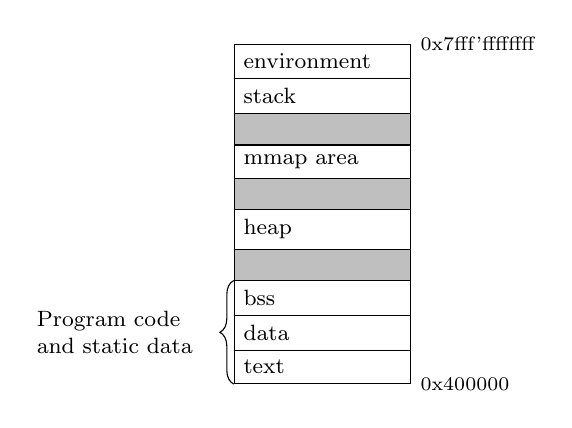
\begin{tikzpicture}[font=\footnotesize]

    % See page 453 in pgf manual
    \node [
      rectangle split, rectangle split parts=10, 
      rectangle split part fill={white, white, lightgray, white, lightgray, white, lightgray, white},
      draw, anchor=center, text width=2cm
    ] (m)
      {
        \nodepart{one}
          environment
        \nodepart{two}
          stack
        \nodepart{four}
          mmap area
        \nodepart{six}
          heap
        \nodepart{eight}
          bss
        \nodepart{nine}
          data
        \nodepart{ten}
          text
      };

    \draw [decorate, decoration={brace, amplitude=5pt}] (m.south west) -- (m.seven split west) 
      node [black, midway, xshift=-1.5cm, text width=2.0cm] 
        { Program code and static data } ;

    \node[right] at (m.north east)
      { \scriptsize{0x7fff'ffffffff} } ;

    \node[right] at (m.south east)
      { \scriptsize{0x400000} } ;

  \end{tikzpicture}
\end{figure}

Text and data sections contain program code and static data respectively.
These regions are mapped towards the low en of the address spectrum, and the virtual addresses of variables allocated here will not change with environment size. 

Note that the initial position of stack will not depend on environment size this way when address randomization (ASLR) is enabled. (TODO: Does it offset from page boundary? That would be good, same alias behavior :)

Addresses of stack allocated variables can vary depending on environment size, while other segments of memory such as text and data remain constant over all environments.

To illustrate how this can cause bias, we revisit the example first presented in~\cite{Mytkowicz:2009:WrongData}, shown in Listing~\ref{lst:loopkernel}. 
This example is interesting for several reasons. 
The bias effects are significant and easily reproducible, while the example code is simple and easy to analyze.
Still, no satisfactory explanation as to what causes bias was given in the original paper.

\begin{lstlisting}[float=h, language=C, caption={Microkernel succeptible to aliasing between static variables and automatic variables for certain environment sizes}, label={lst:loopkernel}, frame=lines]
static int i, j, k;
int main() {
    int g = 0, inc = 1;
    for (; g < 65536; g++) {
        i += inc;
        j += inc;
        k += inc; 
    }
    return 0;
}
\end{lstlisting}

Their program contains five variables, two of which are stack allocated and i, j and k that are statically allocated.
Performance counter measurements of cycle counts are shown for 512 different environment sizes in Figure~\ref{fig:envbias}.
Sampling is done for every 16 byte increment of environment size, covering two 4K periods of addresses.
A finer sampling is not necessary, because the stack is by default aligned to 16 byte.
The program is compiled with GCC using no optimization.
Any optimization would likely disregard most of the function as redundant code, and reduce it to return zero immediately.

There are clearly two worst cases, indicated by significant spikes around the 3100 and 7100 byte offsets.
We analyzed these cases by sampling an extensive set of performance counters and correlating them with cycle counts.
The results show a high number of resource stalls when the spikes occur, indicated by high values for performance counters \small{RESOURCE\_STALLS.ANY}, \small{CYCLE\_ACTIVITY.CYCLES\_LDM\_PENDING}, \small{CYCLE\_ACTIVITY.CYCLE\_NO\_EXECUTE} and \small{RESOURCE\_STALLS.RS}.
We also find that \small{LD\_BLOCKS\_PARTIAL.ADDRESS\_ALIAS} correlates almost perfectly with cycle count, which can explain the high number of resource stalls with false dependency from aliasing.

\subsection{Finding Collisions}
To be able to explain what is happening in this case we need to know the addresses of all variables at run time.
For statically allocated data, memory allocation is decided at compile time.
The location of variables i, j and k can be found by looking at the symbol table in the ELF executable.
Below is an excerpt of \lstinline$readelf -s$.
\begin{lstlisting}[float=h, basicstyle=\small]
37: 000000000060103c    4  (...)  25 i
38: 0000000000601040    4  (...)  25 j
39: 0000000000601044    4  (...)  25 k
\end{lstlisting}

Need to observe run time addresses without introducing any observer effects.
A small amount of assembly code was used to calculate the addresses of each stack allocated variable and output them directly using system calls, without impacting run time addresses.
We find that the spike in cycle count occurs when the address of inc alias with i, where the first spike happens when inc is at 0x7fffffffe03c.
Because the stack is aligned to 16 byte or 4 words, there are a couple of different scenarios that could have been observed here.
Static area is fixed and covers 12 contiguous bytes (3 words) \lstinline$[x|x| |x]$.
Automatic variables occupies 8 contiguous bytes on stack (2 words) [ | |x|x]. 
The space of possible addresses for (inc, g) in this case is (0x7fffffffe03c, 0x7fffffffe038) - n*4096. 
In this scenario, g will never alias with any of the static variables -- as it always covers the 0x8 slot not occupied by either of i, j or k.
An even worse case with respect to the number of alias events is if allocation of static data allows collisions with both stack allocated variables.
This can be achieved by reserving an extra 8 bytes to offset i, j into the 0x8, 0xc slots. 
While this will give significantly more alias counts, it has little effect on the number of cycles executed.

Worst case occurs for precisely one out of 256 possible initial stack addresses in every 4K segment.
Resource stalls are generated because of false dependencies between stack and static data, resulting in worse performance.
The program is \emph{biased} towards environment sizes that avoids this specific stack alignment.


\subsection{Offset to Avoid Aliasing}
Addresses of automatic variables can not be determined statically, because the position of stack at runtime is generally unknown. 
In addition to being offset by environment variables, the stack address can also be perturbed by other factors such as address layout randomization. 
Although one can not easily know if a collision is going to happen for a given environment, one can try to change the program to account for possible alias effects.
The following strategy is a proof of concept of how alias-free code can be generated in this particular case.
If the addresses do alias, branch to an alternative but semantically equivalent code path.
Allocate a new set of variables to avoid aliasing.

\begin{lstlisting}[float=h, language=C, caption={Dynamically detect aliasing case, and avoid by pushing another stack frame.}, label={lst:loopkernel}, frame=lines]
#define ALIAS(a, b) \
    ((((long)&a)&0xfff)==(((long)&b)&0xfff))
static int i, j, k;
int main() {
    int g = 0, inc = 1;
    if (ALIAS(inc, i) || ALIAS(g, i))
        return main();
    for (; g < 65536*10; g++) {
        i += inc;
        j += inc;
        k += inc;
    }
    return 0;
}
\end{lstlisting}



\section{Bias from Heap Allocators}
Address aliasing can be caused by conflicting pairs of load/store operations to any part of memory.
The previous section looked specifically at an example of collision between stack variables and static data.
Another scenario to consider is collisions in heap allocated memory.
In particular, code that operate on pairs of contiguous arrays can be vulnerable to 4K aliasing.
Acquiring dynamic memory at run time is usually done by calling malloc, which takes a number of bytes to allocate and returns a pointer to that area.
A typical malloc implementation uses two different strategies for how to allocate memory.
The \emph{heap} area in virtual memory is used for smaller allocations.
Programs are initially given a small heap area, which the allocator can increase by calling brk or sbrk.
For larger allocations, it is typically faster to use anonymous memory mapping by calling mmap, instead of growing the ``normal'' heap.
The heap starts at a low address close to the data section and grows towards higher addresses. 
Mmap allocates much closer to the stack.
While heap addresses can look like 0x16e30a0 or 0x1723020, pointers returned by mmap can for example be 0x7f0318a8f010 or 0x7f03105d2010.
This distinction is of course unimportant for application developers, as everything is conceptually the same ``heap''.
However, mmap has an interesting property in that allocations will always be page aligned.
The page size is 4096 bytes, meaning two pointers returned by mmap will \emph{always} alias.\footnote{libc's version of malloc adds 16 bytes of medatada at the beginning, therefore every mmap'ed address ends with 0x010}

Consider the function shown in Listing~\ref{lst:conv}.
It computes the convolution between an input array and a fixed five-element kernel, writing the result to another array.
For simplicity, endpoints are not handled.

\pgfplotstableread{bin/convolution.dat}{\convolutiontable}
\begin{figure}[t]
  \caption{Cycle and alias counts for different offsets between input and output arrays in Listing~\ref{lst:conv}. Offset 0 means equal 12 bit address suffix, which is default behavior for mmap allocations. Array size $n=2^{20}$, compiled with -O3. }
  \label{fig:heapalias}
  \begin{tikzpicture}
    \begin{axis}[
        font = \small,
        xlabel=Relative offset in \lstinline!sizeof(float)! bytes,
        cycle list name=black white
      ]
      \addplot table[x expr = \thisrowno{0}, y = cycles:u] \convolutiontable ;
      \addplot table[x expr = \thisrowno{0}, y = r0107:u ] \convolutiontable ;
      \addlegendentry{cycles:u} ;
      \addlegendentry{r0107:u} ;
    \end{axis}
  \end{tikzpicture}
\end{figure}

\begin{lstlisting}[float=t, language=C, caption={Naive implementation of convolution. Highly sensitive to aliasing between input and output arrays.}, label={lst:conv}, frame=lines]
static float k[5]={0.1,0.25,0.3,0.25,0.1};
void conv(int n, float *in, float *out) {
    int i, j;
    for (i = 2; i < n-2; ++i) {
      out[i] = 0;
      for (j = 0; j < 5; ++j)
          out[i] += in[i-2+j] * k[j];
    }
}
\end{lstlisting}


Figure \ref{fig:heapalias} shows how this function behaves when given input with different alignment.
The default behavior for large heap allocations is that both arrays alias.
To force different alignments, we allocate some extra bytes at the end and offset the output pointer argument.

\begin{lstlisting}
output = malloc(n * (sizeof(float) + offset));
conv(n, input, output + offset);
\end{lstlisting}

Listing \ref{lst:conv}, together with a small main method handling the allocation and offset, is compiled with optimization O3 and input size n=$2^{20}$.
Figure \ref{fig:heapalias} plots performance counter statistics for cycle count and 4K alias events over increasing amount of offset.
This is an example of how false dependencies from address aliasing can cause a significant performance hit.
Because large heap allocations always alias, the processor thinks memory accesses to input[i] potentially conflicts with output[i], stalling the pipeline.
By manually adjusting the alignment of one input buffer, cycle count can be reduced by more than 50\% (verify).
This is a speedup on top of compiler optimization O3, which is not able to account for aliasing effects.

It is perhaps unfair to assume the compiler can fix this when only given a generic optimization flag, as aliasing effects is (presumably) an Intel-specific issue.
You might also wamt to utilize the C99 keyword restrict to explicitly tell the compiler that the buffers are disjoint in memory.

\begin{lstlisting}[language=C]
void conv( int n,
            const float * restrict in,
            const float * restrict out );
\end{lstlisting}

Even with the updated signature compiled with -O3 -march=native, there is still room for improvement by inserting manual offsets.


\subsection{Behavior of other Allocators}
Addresses of dynamic memory at run time is governed by the particular heap allocator used.
Like the contents of environment varialbes, the exact operation of heap allocation can typically not be known ahead of time.
For the code examples we present in C, the dynamic linker will resolve malloc to whichever version of libc is available on the system.
In other words, it is part of the environment, and a potential source of measurement bias.
(table, todo)



\section{Performance Impact in Numeric Applications}

Basic Linear Algebra Subroutines (BLAS), is the de facto standard API for high performance linear algebra routines.
The functionality is divided into three categories: 

\begin{description}
  \item{Level 1} Scalar and vector operations, such as dot product and vector addition.
  \item{Level 2} Matrix-vector operations, such as gemv for general matrix-vector multiplication.
  \item{Level 3} Matrix-matrix operations, including the widely applied gemm routine for general matrix-matrix multiplication. 
\end{description}

Many highly optimized implementations of BLAS exists, ATLAS being a widely used and open source alternative. One of the key features of ATLAS is that it uses automatic tuning to optimize for cache efficiency [Whaley:2000:ATLAS]. 

We use the currently latest stable version 3.10.1 of ATLAS, built as a shared library from source.
The automatic tuning happens during the build process.
A series of test programs are run to determine cache edges and other properties of the hardware, which in turn affects the resulting binary. 

Carefully monitoring cache is particularly important in this case study, as BLAS performance heavily relies on cache efficiency.
Relevant performance statistics for cache hit ratios will be considered to rule out cache as the cause of any bias effects.

The idea is to reproduce similar scenarios to what we saw in Section ?, where aliasing was caused by linear accesses to pairs of aligned heap allocated data.
Functions operating on vectors, from BLAS Level 1 or 2, seems most likely to have potential for similar characteristics.
Using heap allocated memory, address aliasing is an artifact of the allocator used.
With different versions or configurations of memory allocators, any performance impact from aliasing can qualify as measurement bias.
In the following sections, we will study bias from address aliasing in the Level 2 function gemv specifically, which computes matrix-vector multiplication.

Consider matrix-vector multiplication of the form $\boldsymbol{y} = A\boldsymbol{x} + \boldsymbol{b}$ . Let A be of size $M \times N$, where M is the number of rows. 

$
\left[\begin{array}{ccccc}
a_{0,0} & a_{0,1} &  &  & a_{0,N}\\
a_{1,0}\\
 &  &  & \ddots\\
a_{M,0} &  &  &  & a_{M,N}
\end{array}\right]\left[\begin{array}{c}
x_{0}\\
x_{1}\\
\vdots\\
\\
x_{N}
\end{array}\right]=\left[\begin{array}{c}
y_{0}\\
y_{1}\\
\vdots\\
y_{M}
\end{array}\right]
$

The corresponding BLAS function is the level 2 gemv routine, computing the more general matrix-vector product given as $\boldsymbol{y} = \alpha\text{op}\left(A\right)\boldsymbol{x} + \beta\boldsymbol{y}$
Here, $\alpha$ and $\beta$ are constants, and $\text{op}\left(A\right)$ is an optional transpose or complex conjugate of the matrix. 
We set $\alpha = 1$, $\beta = 0$ and $\text{op} \left(A\right) = A$ to reduce the formula to $\boldsymbol{y}=A\boldsymbol{x}$.

To better be able to assess the effects of aliasing, the call to gemv needs to be isolated. 
We make two benchmarks, one with iteration count $K = 1$ and another with $K = 101$.
An approximation of the cost for a single invocation of dgemv can be expressed as 
$$
t_{\text{estimate}}=\frac{t_{K=101}-t_{K=1}}{100}
$$
where t represents some metric, such as the number of cycles.
Subtracting the $K = 1$ run removes the constant overhead from the $K = 101$ run.
Dividing by $100$ averages the values from the remaining iterations.
Other iteration counts could have been used as well.

\begin{table*}[t]
  \caption{Estimated cost of invoking cblas\_dgemv with a matrix size $8192 \times 8192$}
  \label{tab:atlas8k}
  \small
  \centering
  \begin{tabular}{l r r r}
    \toprule
      & (0x010, 0x010, 0x020) & (0x010, 0x010, 0x0b0) & (0x010, 0x140, 0x150) \\
    \midrule
    CPU\_CLK\_UNHALTED.THREAD\_P & 162,926,895 & 152,151,263 & 144,583,160 \\
    LD\_BLOCKS\_PARTIAL.ADDRESS\_ALIAS & \textbf{68,408,790} & \textbf{5,154,981} & \textbf{2,919} \\

    MEM\_UOPS\_RETIRED.ALL.LOADS & 100,701,777 & 100,702,138 & 100,701,752 \\
    MEM\_LOAD\_UOPS\_RETIRED.HIT\_LFB & 31,628,539 & 32,495,287 & 29,853,850 \\
    MEM\_LOAD\_UOPS\_RETIRED.L1\_HIT & 68,309,447 & 65,625,881 & 69,387,368 \\
    MEM\_LOAD\_UOPS\_RETIRED.L2\_HIT & 711,973 & 1,540,956 & 864,720 \\
    MEM\_LOAD\_UOPS\_RETIRED.L3\_HIT & 154,345 & 651,985 & 363,331 \\
    MEM\_LOAD\_UOPS\_RETIRED.L3\_MISS & 106,313 & 350,449 & 295,235 \\
    MEM\_UOPS\_RETIRED.ALL.STORES & 33,562,692 & 33,562,692 & 33,562,692 \\

    LOAD\_HIT\_PRE.HW\_PF & 42,914,191 & 47,315,935 & 59,211,320 \\
    \bottomrule
  \end{tabular}
\end{table*}

Notes: 
 - More BR\_INST.COND.TAKEN taken in case (a), but number of retired instructions are the same. Suggests replays of instructions.
 - Inverse HW prefetch numbers from masters


Estimated performance counter statistics for each of the three heap address configurations are shown in Table [?tab:gemv-estimate].
In addition to cycle count and alias events, a number of relevant metrics related to cache activity are also included.
Notice that almost all load micro-ops are served by either the line fill buffer or L1 cache in all cases.
Only a small amount of loads come from L2, and almost none from L3.
The hit rate for L1 actually decreases somewhat (considering LFB as well) with better execution time.
This could be explained by less time for prefetchers to feed the L1 cache with data.
The hardware prefetch counter indicates more hits in cases a and b.
Again, we find that cache efficiency does not explain the performance cliffs we observe. 

Our results show that address aliasing between matrix and vector heap buffers can significantly impact performance of dgemv in ATLAS.
Variations in heap addresses alone can give a speedup of more than 30 \%.


\subsection{Dealing with Aliasing}
For the particular case we investigated, a good heuristic is to align heap segments “far apart” within the 4 KiB area of 12 bit suffixes.
More specifically, it appears that address suffixes of A and $\boldsymbol{y}$ are the most important to separate.

As discussed in section [x], aliasing cases like these can be accounted for in software using padding techniques.
A possible run time solution to adjust heap addresses can be realized as follows:

\begin{itemize}
  \item Allocate some extra space for one of the vectors when calling malloc, for instance sizeof(double) * (M + 0x100) for $\boldsymbol{y}$.

  \item Check the returned pointers for potential alias, i.e. the difference between \&A and \&y. Offset using pointer arithmetic into the array with extra padding at the end, i.e. y += 0x100. 
\end{itemize}

Another option is to explicitly account for “worst cases” in the implementation of routines that are vulnerable to aliasing.
Addresses can be explicitly checked for potential conflicts in cblas\_dgemv, and if possible branch to code that will not suffer from aliasing. 


\section{Conclusions}
Any change to virtual memory layout of data can potentially introduce bias effects from address aliasing. 
We find that compilers, even when provided with architecture specific optimization flags, still generates code that suffers from aliasing. 
Typical heap allocators return page-aligned memory by default, which is the worst case with respect to aliasing for many algorithms.
Despite recommendations from Intel, we are not aware of any allocators that specifically addresses this issue.


%\onecolumn

\bibliographystyle{plain}
\bibliography{references}

\end{document}
